\documentclass[11pt]{article}
\pdfinfoomitdate=1\pdftrailerid{}
\usepackage[letterpaper,margin=.7in,headheight=15pt,headsep=18pt,footskip=24pt]{geometry}
\usepackage[T1]{fontenc}\usepackage{lmodern,amsmath,amssymb,array,booktabs,fancyhdr,hyperref,tikz}
\renewcommand{\familydefault}{\sfdefault}\setlength{\parindent}{0pt}\setlength{\parskip}{7pt}
\pagestyle{fancy}\fancyhf{}\fancyhead[L]{\small Week 97 / Square remainders / Facilitator guide}
\fancyfoot[L]{\scriptsize Bellingham Math Circle / Week 97 / W97-FAC-v2}\fancyfoot[R]{\thepage}
\newcommand{\head}[1]{\par\textbf{\large #1}\par}
\newcommand{\sub}[1]{\par\textbf{#1}\par}
\begin{document}
\head{Mathematical overview: what this investigation establishes}
\textbf{The operation.} An input $n$ is a nonnegative whole-number side length. Its square has $n^2$ counters. Remove complete bundles of a positive size $m$ until fewer than $m$ counters remain. The output is the unique remainder $r$ with $0\le r<m$. Both input 0 and output 0 participate. The input is a side length, not an area.

\textbf{A finite search can cover every input.} Replacing an input by another with the same remainder modulo $m$ leaves its square output unchanged. In particular, inputs $0,1,\ldots,m-1$ produce every possible output, even if arbitrarily large inputs are allowed. If $n=mq+s$, then
\[
 n^2-s^2=mq(mq+2s),\qquad 0\le s<m.
\]
The removed area is a multiple of $m$. Page 4 gives a rectangular-strip explanation suitable for a whiteboard.

\textbf{Prime square outputs come in pairs.} For an odd prime $p$ and inputs $x,y$ in $0,\ldots,p-1$, the square outputs agree exactly when $x=y$ or $x+y=p$. Zero is produced only by input 0. Every occurring nonzero output is produced by exactly two inputs, $x$ and $p-x$. There are therefore $(p-1)/2$ nonzero square outputs, and $(p+1)/2$ outputs including zero. The proof uses the fact that a prime dividing a product divides a factor; page 5 proves and applies that fact.

\textbf{Composite sizes change the information.} With bundles of 8, output 1 has four possible inputs in $0,\ldots,7$. With bundles of 9, output 0 has three. With bundles of 15, outputs 1 and 4 each have four possible inputs. These examples refute a universal two-input rule. They do not say that every composite has the same behavior or that every composite gives several inputs for output 0.

\textbf{Optional multiplicative continuation.} For an odd prime, classify the \emph{nonzero} remainders as squares or nonsquares. Square times square is square, square times nonsquare is nonsquare, and nonsquare times nonsquare is square. Products are reduced modulo the same prime. Page 6 explains the assumptions and proof; zero is excluded from this classification.

\textbf{Discovery and readiness.} Children first make and reverse a concrete operation, then discover that a single exact output may leave several inputs possible: two inputs for each nonzero output with bundles of 3, 5, 7 and 11; three or four for some outputs with bundles of 8, 9 and 15; and no new output from inputs past $m-1$. Grades 3--5 are approximate: entry requires square arrays, equal bundles, supported multiplication and comparing small collections. Systematic comparison and universal arguments are later work. Problems 1--2 are a complete first route; Problems 3--6 and the optional product investigation can occupy return visits. There is no K--1 packet (page 2 gives an adult-led K--1 route) and no assumption that Week 96 has been completed. Experiments suggest patterns; exhaustive lists prove finite claims; the general identities and prime argument establish the universal claims.
\newpage
\head{Preparation, launch and a first route}
\textbf{Status.} Unpiloted. Printing, material preparation, procedures and timings have not been physically rehearsed. The suggestions below are a proposed route, not classroom evidence.

\textbf{Staffing and materials.} One adult per participating table. The four third graders can work in two pairs; the two fourth graders and fifth grader can rotate maker, guesser and checker. The K--1 table takes the K--1 route below with its adult. For each pair provide 64 counters or square tiles, a whiteboard and pen, scrap paper and about 16 reusable input cards. Write output labels on scrap paper if children choose to sort their results. There is no required cutout deck or exact material fit. Reuse the counters for successive inputs; do not build every square simultaneously.

Allow about 10 minutes to count kits and mark cards. Print US Letter, single-sided, Actual Size. For a first visit, print student pages 1--2, with page 3 available for a ready group. Print pages 5 and 6 together: Problem 6's check with bundles of 15 needs $11\times11$ to $14\times14$, which page 5 prints. The later pages include square products so children need not calculate or physically build squares of 196 counters. Offer a multiplication reference. If finding remainders becomes the bottleneck, an adult may record a child's repeated subtraction or help make a multiples strip; the child should still choose cases and decide what the collection says.

\sub{Launch together: about 5 minutes after movement}
Let children handle the counters first. Make the printed input-3 example: a $3\times3$ square, nine counters in all. Keep those same nine counters in view. Put four in one loop, four in another, and leave one outside. No complete bundle of 4 remains, so the output is 1. Show input 0 with no counters: its output is also allowed and is 0. Ask a child to make a legal attempt before distributing starting tasks.

Now read the small printed collection for \emph{bundles of 4 and inputs 0--3}. The top row names inputs and the bottom row their outputs. Output 1 could hide input 1 or input 3: two possibilities. The different outputs in the whole collection are 0 and 1. These are two different questions about a collection. This worked convention prepares the task without supplying its bundle-5 answers. Children may draw, arrange input cards under output labels, or choose their own records.

\sub{A manageable first visit}
Allow 10--15 minutes for Problem 1 and 15--20 for the partner game in Problem 2, with time to compare the collections and share what a remainder reveals. In the partner game, the maker hides both the chosen input and the square: the partner looks away or a sheet screens the construction. Announce only the output. In the group of three, rotate roles after each secret. A guess is complete when it names every allowed input, not merely the maker's actual one.

For a further 10--15 minutes, compare one new bundle size from Problem 3. A whole-table collection can pool cases; each child need not copy every calculation. End with one useful collection and a question to return to. Problems 3--4 can fill another visit, and Problems 5--6 another. A child still engaged in sorting small squares need not advance to an abstract proof. Reading aloud or recording a child's explanation is routine support; adults organizing every case or making all comparisons is a readiness signal to return to a smaller concrete collection.

\textbf{K--1 route (adult-led, no packet, about 15 minutes).} After the launch, the K--1 table builds the squares $1\times1$ to $5\times5$ with counters; the parent reads and records. Put each square's counters into groups of 3 and ask: ``Can a square leave 2?'' Then try groups of 4: ``Can a square leave 2 or 3?'' Key in plain words: with groups of 3 the squares leave 1, 1, 0, 1, 1, so never 2; with groups of 4 they leave 1, 0, 1, 0, 1, so never 2 or 3. That K--1 children sustain this is a prediction; it is untested.
\newpage
\head{Problems 1--3: complete collections and answers}
In the tables below, braces contain \emph{input side lengths}. The label to the left of each brace is an output. Missing outputs in $0,\ldots,m-1$ never occur for the stated input range. Each finite range includes both endpoints.

\begin{center}\renewcommand{\arraystretch}{1.25}
\begin{tabular}{c p{11.4cm}}
\toprule Bundle size & Output: all possible inputs from 0 to one less than the size\\\midrule
5 & $0:\{0\};\quad1:\{1,4\};\quad4:\{2,3\}$\\
7 & $0:\{0\};\quad1:\{1,6\};\quad2:\{3,4\};\quad4:\{2,5\}$\\
8 & $0:\{0,4\};\quad1:\{1,3,5,7\};\quad4:\{2,6\}$\\
9 & $0:\{0,3,6\};\quad1:\{1,8\};\quad4:\{2,7\};\quad7:\{4,5\}$\\\bottomrule
\end{tabular}\end{center}

\sub{Problem 1, page 1: same output, different inputs}
For bundles of 5, the different-input pairs are $\{1,4\}$ and $\{2,3\}$. Their outputs are 1 and 4 respectively. Input 0 has no different partner. Outputs 2 and 3 cannot occur. Checking the five allowed inputs makes a complete proof of this finite claim. It does not yet settle inputs above 4.

\emph{Hints, only if needed:} ask a child to show one square, put aside all full bundles, and leave the remainder visible. Keep one input card beside its output rather than several simultaneous tallies. If 0 is omitted, ask what happens when the square has no counters. If input 3 is treated as three counters, return to the side-length label in the worked square.

\sub{Problem 2, page 2: what the output reveals}
For bundles of 7, output 0 forces input 0. Outputs 1, 2 and 4 each hide two inputs, as the table shows. Thus those three outputs tie for the most possibilities; 0 has the fewest. The question specifies outputs that occur, so the absent outputs 3, 5 and 6 are not answers to the minimum question.

The partner may be unable to name the actual secret, even with perfect calculation. Naming the complete collection is success. The exact observation loses information because several inputs share it. This is an inverse problem: recover what can be known about an input from an observed result. No random choice or measurement error is required.

\emph{Hint:} if a child finds one possible input and stops, the maker can ask whether another allowed square has that output. If children compare output numbers instead of numbers of possibilities, return to the small bundle-4 example. Do not announce the opposite-input pairing before it arises from their work.

\sub{Problem 3, page 3: changing the bundle size}
For 7, outputs 1, 2 and 4 each have the maximum of two inputs. For 8, output 1 has four inputs, the unique maximum. For 9, output 0 has three inputs, the unique maximum. Bundle size 8 therefore has the output that hides the most inputs. A follow-up to ask aloud: can output 0 hide more than one input? Yes, for 8 and 9 (page 1 already shows 0 and 2 with bundles of 4).

\emph{Hints and pacing:} begin with one new size and preserve its input cards for comparison. Two children can check different inputs and pool results. Ask where an unchecked input could still fit if the collection is incomplete. Once the largest collection is found, a complete catalog is what rules out a still larger one. The contrast concerns the structure of equal-output groups; the larger output label need not mean more possible inputs.
\newpage
\head{Problems 4--5: four-way ambiguity and every input}
\sub{Problem 4, page 4: bundles of 15}
The inputs producing output 1 are $1,4,11,14$. Their squares are $1,16,121,196$, each one above a multiple of 15. No output hides more than four allowed inputs; output 4 ties. The full inventory is:
\[
\begin{array}{c|l@{\qquad}c|l}
\text{output}&\text{inputs}&\text{output}&\text{inputs}\\\hline
0&0&1&1,4,11,14\\
4&2,7,8,13&6&6,9\\
9&3,12&10&5,10
\end{array}
\]
The six collection sizes are $1,4,4,2,2,2$; together they contain all 15 inputs. Inspecting only output 1 would not settle whether another output hides more. A table or arrangement of cards makes the completeness check visible. Supplied square facts support the arithmetic; physical construction of every large square is unnecessary.

\sub{Problem 5, page 5: why bigger inputs give no new output}
For bundles of 7, every input has the same square output as one of $0,\ldots,6$. The only outputs are $0,1,2,4$. The printed inputs $7,\ldots,15$ give outputs $0,1,4,2,2,4,1,0,1$. These examples suggest the claim; the following argument covers all inputs.

First demonstrate one unchanged square. Input 10 has area 100. Remove seven full columns, area 70. From the remaining $3\times10$ rectangle, remove seven full rows, area 21. A $3\times3$ square, area 9, remains. Both removed rectangles split into bundles of 7, so 100 and 9 leave the same output, 2.

\begin{center}
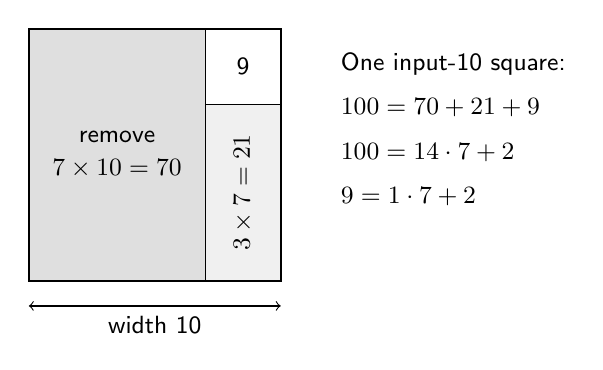
\begin{tikzpicture}[x=.32cm,y=.32cm]
\fill[gray!25] (0,0) rectangle(7,10);\fill[gray!12] (7,0) rectangle(10,7);
\draw[thick] (0,0) rectangle(10,10);\draw (7,0)--(7,10);\draw (7,7)--(10,7);
\node[align=center] at(3.5,5){\small remove\\\small $7\times10=70$};
\node[rotate=90] at(8.5,3.5){\small $3\times7=21$};
\node at(8.5,8.5){\small 9};
\draw[<->] (0,-1)--node[below]{\small width 10}(10,-1);
\node[align=left,anchor=west] at(12,6){\small One input-10 square:\\[4pt]\small $100=70+21+9$\\[4pt]\small $100=14\cdot7+2$\\[4pt]\small $9=1\cdot7+2$};
\end{tikzpicture}
\end{center}

For any $n=7q+s$, $0\le s<7$, remove $7q$ columns from the $n\times n$ square, then $7q$ rows from the remaining $s\times n$ rectangle. The removed areas are $7qn$ and $7qs$, both multiples of 7. The remaining square is $s\times s$. This works even when $s=0$ or $q=0$, when a region is empty. It proves the identity on page 1 and works for any positive bundle size.

\emph{Hints:} compare inputs 3 and 10 using a drawing before general letters. Ask what adding seven to a side adds to the area. Avoid confusing seven rows with seven counters. A child may give another sound area or arithmetic argument; testing still more examples alone does not settle every input.
\newpage
\head{Problem 6: the odd-prime rule and its proof}
Before this continuation, connect the vocabulary to the action: a positive divisor of a whole number makes exact equal bundles with nothing left. For example, 3 divides 12 because four bundles of 3 use all 12 counters.

For bundle sizes $3,5,7,11$, the respective numbers of outputs including zero are $2,3,4,6$. The inventories for 5 and 7 are on page 3. The other two are:
\[
\begin{array}{c|l}
3&0:\{0\};\quad1:\{1,2\}\\[3pt]
11&0:\{0\};\quad1:\{1,10\};\quad3:\{5,6\};\quad4:\{2,9\};\\
&5:\{4,7\};\quad9:\{3,8\}
\end{array}
\]
The conjecture is $(p+1)/2$ outputs for every odd prime $p$: one output for input 0 and one for each pair of nonzero opposite inputs. Examples establish the four finite counts; the prime argument establishes the general rule.

\sub{Why the pairing is exact}
\noindent\begin{minipage}[c]{0.6\linewidth}
\emph{With counters.} Take a $2\times2$ corner off a $5\times5$ square. The L left, 21 counters, is a $3\times5$ strip and a $3\times2$ strip; laid end to end they make a $3\times7$ rectangle, three bundles of 7, so inputs 5 and 2 share an output with bundles of 7. In general, taking a $y\times y$ corner off an $x\times x$ square leaves an L that re-forms as an $(x-y)\times(x+y)$ rectangle. With bundles of 7 it is whole bundles when it is empty ($x=y$) or a side is 7 ($x+y=7$); the prime fact below says only then. Grades 4--5 can explain Problem 6 this way.
\end{minipage}\hfill
\begin{minipage}[c]{0.37\linewidth}\centering
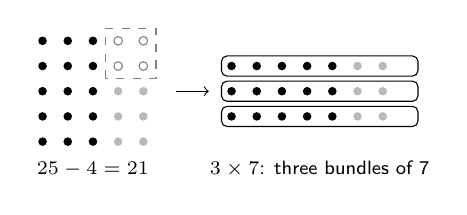
\begin{tikzpicture}[x=0.32cm,y=0.32cm]
\foreach \c in {0,1,2} \foreach \r in {0,...,4} {\fill (\c,\r) circle (0.17);}
\foreach \c in {3,4} \foreach \r in {0,1,2} {\fill[gray!55] (\c,\r) circle (0.17);}
\foreach \c in {3,4} \foreach \r in {3,4} {\draw[gray] (\c,\r) circle (0.17);}
\draw[gray,dashed] (2.5,2.5) rectangle (4.5,4.5);
\node[font=\scriptsize] at (2,-1.1) {$25-4=21$};
\draw[->] (5.3,2)--(6.6,2);
\foreach \c in {0,...,4} \foreach \r in {0,1,2} {\fill (7.5+\c,1+\r) circle (0.17);}
\foreach \c in {5,6} \foreach \r in {0,1,2} {\fill[gray!55] (7.5+\c,1+\r) circle (0.17);}
\foreach \r in {0,1,2} {\draw[rounded corners=2pt] (7.1,0.6+\r) rectangle (14.9,1.4+\r);}
\node[font=\scriptsize] at (11,-1.1) {$3\times7$: three bundles of 7};
\end{tikzpicture}
\end{minipage}

For inputs $x,y$ in $0,\ldots,p-1$, equal outputs mean their squares differ by a multiple of $p$. Factor the difference: $x^2-y^2=(x-y)(x+y)$. A prime dividing a product divides a factor. Thus $p$ divides $x-y$ or $x+y$. Since $|x-y|<p$, the first possibility gives $x=y$. If the inputs are distinct, their sum is positive and less than $2p$, so the second gives $x+y=p$. Conversely equal inputs or inputs summing to $p$ always have equal square outputs.

Zero is alone, since $p\mid x^2$ implies $p\mid x$. Every nonzero input $x$ pairs with $p-x$, and these are different because $p$ is odd. No two pairs share an output, by the same argument. The $p-1$ nonzero inputs form $(p-1)/2$ pairs; adding zero gives $(p+1)/2$ outputs. This proves both that the proposed pairs work and that no extra collisions were missed.

\sub{Adult proof support: why a prime divides a factor}
If prime $p$ does not divide $a$, their greatest common divisor is 1. The Euclidean algorithm gives integers $u,v$ with $ua+vp=1$. Multiplying by $b$ gives $b=uab+vpb$. If $p$ divides $ab$, both terms on the right are divisible by $p$, so $p$ divides $b$.

For completeness, the linear-combination fact can be proved without assuming it: choose the least positive integer $d$ of the form $ua+vp$. The remainder on dividing either $a$ or $p$ by $d$ is again such a combination, so minimality forces that remainder to be 0. Thus $d$ divides both. Since $p$ is prime and does not divide $a$, $d=1$. This adult argument is a later explanation, not a prerequisite for the concrete activity.

\sub{What fails for the listed composite sizes}
Actual counts for $8,9,15$ are $3,4,6$, not $(m+1)/2$. Size 8 also lies outside the \emph{odd} hypothesis. More revealing are non-opposite collisions: inputs 1 and 3 for size 8, 0 and 3 for size 9, and 1 and 4 for size 15. For example, 15 divides $(4-1)(4+1)=3\cdot5$, although it divides neither factor. The prime-divides-a-product step is unavailable. The square's remainder still depends only on the input remainder; that earlier fact needs no primality.

\emph{Readiness and hints:} on a return visit, lay out the prime-size input cards and look for partners. Ask whether every input has been placed and whether distinct pairs could still share an output. Introduce the factorization only when children have a conjecture to explain. A facilitated proof can extend across visits; children who can fully justify one finite catalog have already done substantive mathematics.
\newpage
\head{Optional return visit: multiply square-output classes}
This is a new investigation with the familiar bundle operation. For bundles of 7, the nonzero square outputs are $Q=\{1,2,4\}$; the other nonzero remainders are $N=\{3,5,6\}$. These are \emph{output classes}, not collections of secret side lengths. Leave zero out. Write the six labels on cards, sort them into these two groups, then choose two labels, multiply them, remove bundles of 7 and sort the leftover into a group.

Give one complete operation before asking children to vary it: choose labels 3 and 5, make a $3\times5$ rectangle with 15 counters, remove two bundles of 7, and leave 1. Both chosen labels were in $N$; the output is in $Q$. This uses a rectangle for multiplication, not the square-input operation. Children can explore which group a product lands in, compare different choices, and seek a rule. Six labels and at most 36 counters keep the entry concrete; explanations can occupy another visit.

\begin{center}\renewcommand{\arraystretch}{1.2}
\begin{tabular}{c|cc}
Product class & $Q$ & $N$\\\hline
$Q$ & $Q$ & $N$\\
$N$ & $N$ & $Q$
\end{tabular}\end{center}
Examples modulo 7: $2\cdot4=8$ leaves 1; $2\cdot3=6$ leaves 6; $3\cdot5=15$ leaves 1. The table predicts the class, not the exact output. A complete finite table settles size 7. The following argument proves the same class rule for every odd prime.

\sub{Why it works for every odd prime}
Nonzero multiplication modulo a prime is cancellable: if $ab$ and $ac$ agree, the prime divides $a(b-c)$; since it does not divide $a$, it divides $b-c$. Multiplication by a fixed nonzero label therefore permutes the $p-1$ nonzero labels. In particular some label multiplies it to 1, its inverse.

Products of nonzero squares are squares, since $s^2t^2=(st)^2$. Inverses of squares are squares: if $st$ has remainder 1, then $s^2t^2$ does too. Fix a nonsquare $a$. Multiplying every square label by $a$ gives distinct nonsquares: if $aq$ were square for square $q$, multiplying by the square inverse of $q$ would make $a$ square. There are exactly $(p-1)/2$ squares and the same number of nonsquares, so this list contains every nonsquare. Hence any nonsquare $b$ is $aq$ for some square $q$. Then $ab=a^2q$ is square. This proves all three product cases, with zero excluded throughout. It is not asserted for arbitrary composite sizes.

\sub{Connections, sources and evidence}
Week 96's prime bags and this packet meet at the prime-divides-a-product lemma; the present questions concern square outputs and information lost by an exact observation. Week 4's multiplication portraits and Atlas AD-11's four-symbol field are different investigations. The organizer's earlier square arrays provide a familiar action, not an assumed prerequisite visit.

Conrad, \emph{Modular Arithmetic}, \S3, PDF pp. 3--4, supplies remainder arithmetic; \emph{Quadratic Residue Patterns Modulo a Prime}, introduction, PDF p. 1, gives the nonzero-square convention and prime count. See \texttt{SOURCES.md} for URLs, overlap details and teaching evidence from \emph{Math Circle by the Bay}, preface pp. viii--x. All tasks and diagrams are newly authored.

The independent checker verifies printed data, finite collections and prime examples; the arguments above establish the universal statements. Every final student and guide page has been visually inspected; an independent final-pair review is recorded with the package. Digital checks do not establish physical readiness or classroom success. Record actual use, where children needed help, and questions they want to continue.
\end{document}
